\section{Variazione linguaggio di programmazione } 
\hypertarget{section::\theHsection} 
Siccome per la parte di sviluppo della WebApp si è reso necessario utilizzare il linguaggio Javascript, la struttura e l'architettura del software sono state riviste al fine di utilizzare gli strumenti adatti allo sviluppo con tale linguaggio. Rimangono invariati rispetto a prima gli Use Cases, i requisisti funzionali del progetto e l'architettura hardware. Subisce invece variazioni l'architettura Software (deployment, component e class diagram). \autocite[\protect\label{BillNeil2009}][]{BillNeil2009}

\begin{figure}[htp]
\centering
{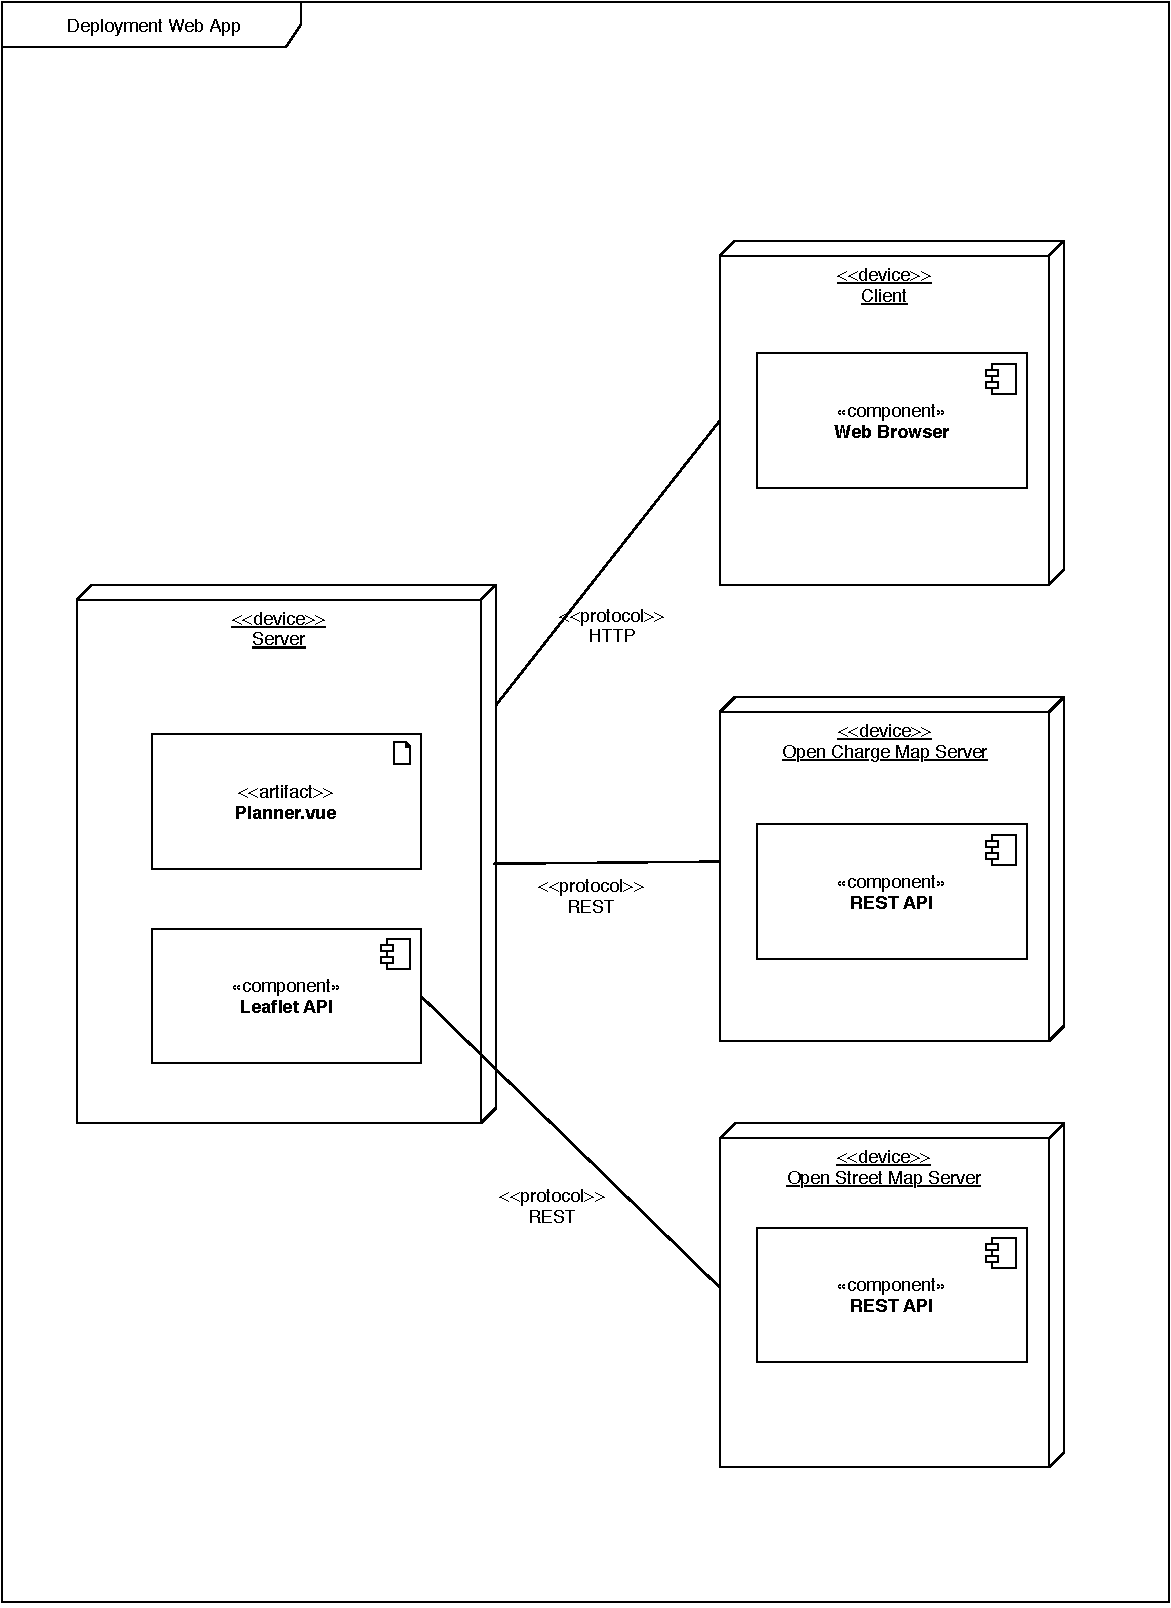
\includegraphics[scale=0.7]{Immagini/Deployment_Diagram_JS.pdf}}
\caption{Template Deployment Diagram}
\end{figure}

Il nuovo deployment diagram si presenta come mostrato in Figura 7.1. Sono presenti 4 device:

device Server che contiene il file Planner.vue che dovrà contenere il software sviluppato, la componente Leaflet API che avrà il compito di comunicare con le API di Open Street Map Server tramite protocollo REST.
Inoltre servirà utilizzare il device Open Charge Map Server e il device Client per lo scaricamento della posizione delle colonnine sulla mappa e la visualizzazione della WebApp sul pc come nel Deploy precedente.

\section {Template} \hypertarget{section::\theHsection}
Per lo sviluppo del software è stato sviluppato una parte di codice in HTML dove vengono definite le tre Textbox visualizzate a schermo, i due bottoni di Search e Reset e la visualizzazione della mappa a schermo centrata all'apertura sulla cartina geografica dell'Italia. \autocite[\protect\label{Sydik2007}][]{Sydik2007}

Per la parte puramente grafica invece è presente un CSS che inserisce nel sito gli elementi grafici visualizzati dall'utente che utilizza il software. \autocite[\protect\label{RobsonFreeman2012}][]{RobsonFreeman2012}

\section{Progettazione dei Test} 
\hypertarget{section::\theHsection}
Abbiamo provveduto alla progettazione dei test relativi a questa iterazione. Sappiamo che la nostra pagina web disporrà di campi in cui l'utente dovrà inserire dei valori e di pulsanti che potrà cliccare. Ci serve quindi un caso di test per questi elementi per assicurarsi che i valori inseriti vengano effettivamente ricevuti e che il click dei pulsanti chiami le relative funzioni: main() se viene cliccato il tasto "Search" e reset() se viene cliccato il tasto "Reset". \autocite[\protect\label{GoodmanMorrisonNovitskiRayl1996}][]{GoodmanMorrisonNovitskiRayl1996}


\section{Template Sequence Diagram}
\hypertarget{section::\theHsection}
Il diagramma di sequenza mostra come a partire da un attore, nel nostro caso un utente (User), il software evolve al fine di restituire all'utente un risultato che in questo caso specifico è rappresentato dalla visualizzazione su mappa del percorso con le fermate alle postazioni di ricarica.

Un utente inserisce l'url nel proprio Browser Web e questi restituirà l'Homepage del sito.
Una volta che l'utente inserisce i dati richiesti questi vengono inviati all'algoritmo scritto in Javascript, che a sua volta invierà una richiesta all'API Leaflet che avrà il compito di interrogare il database delle mappe di Open Street Map e restituire all'algoritmo il percorso dal punto di partenza a quello di destinazione.
L'algoritmo prenderà queste mappe e calcolerà quando è meglio fermarsi per ricaricare il veicolo elettrico, scegliendo tra le possibili colonnine sul percorso.
Dopodichè restituirà l'intero percorso dal punto di partenza a quello di destinazione all'utente con le eventuali fermate da effettuare. \autocite[\protect\label{RichardsonRuby2007}][]{RichardsonRuby2007}

\begin{figure}[H]
\centering
{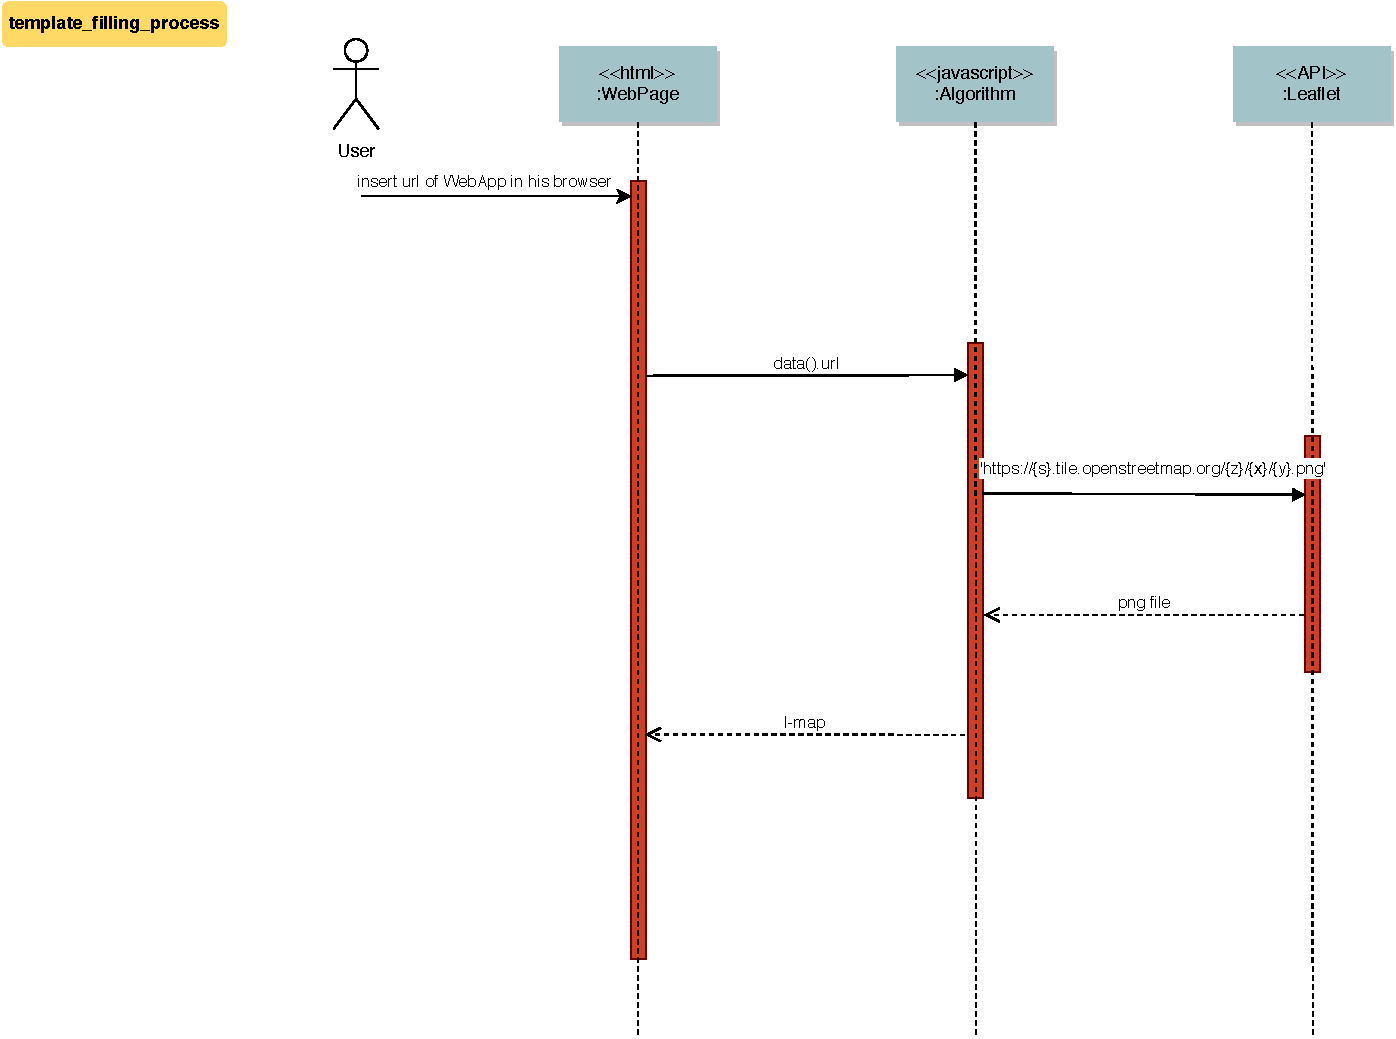
\includegraphics[scale=0.55]{Immagini/Template_SequenceDiagram.pdf}}
\caption{Template Sequence Diagram}
\end{figure}

\section{Risultato dei Test}
\hypertarget{section::\theHsection}
Per concludere questa iterazione presentiamo i risultati dei test che avevamo in precedenza definito. Come si può vedere dalla figura è stata eseguita una suite contente 4 test che hanno avuto tutti esito positivo.

\begin{figure}[H]
\centering
{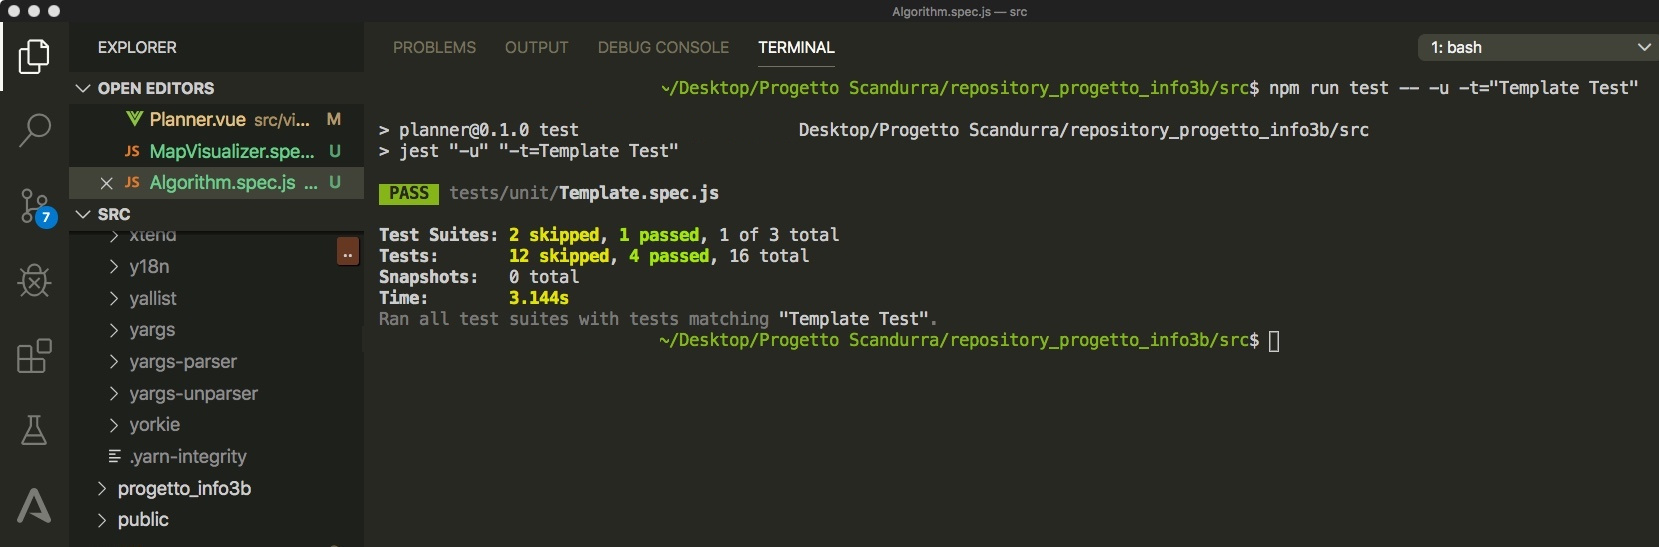
\includegraphics[scale=1]{Immagini/TestTemplate.jpeg}}
\caption{Test iterazione 2}
\end{figure}

